
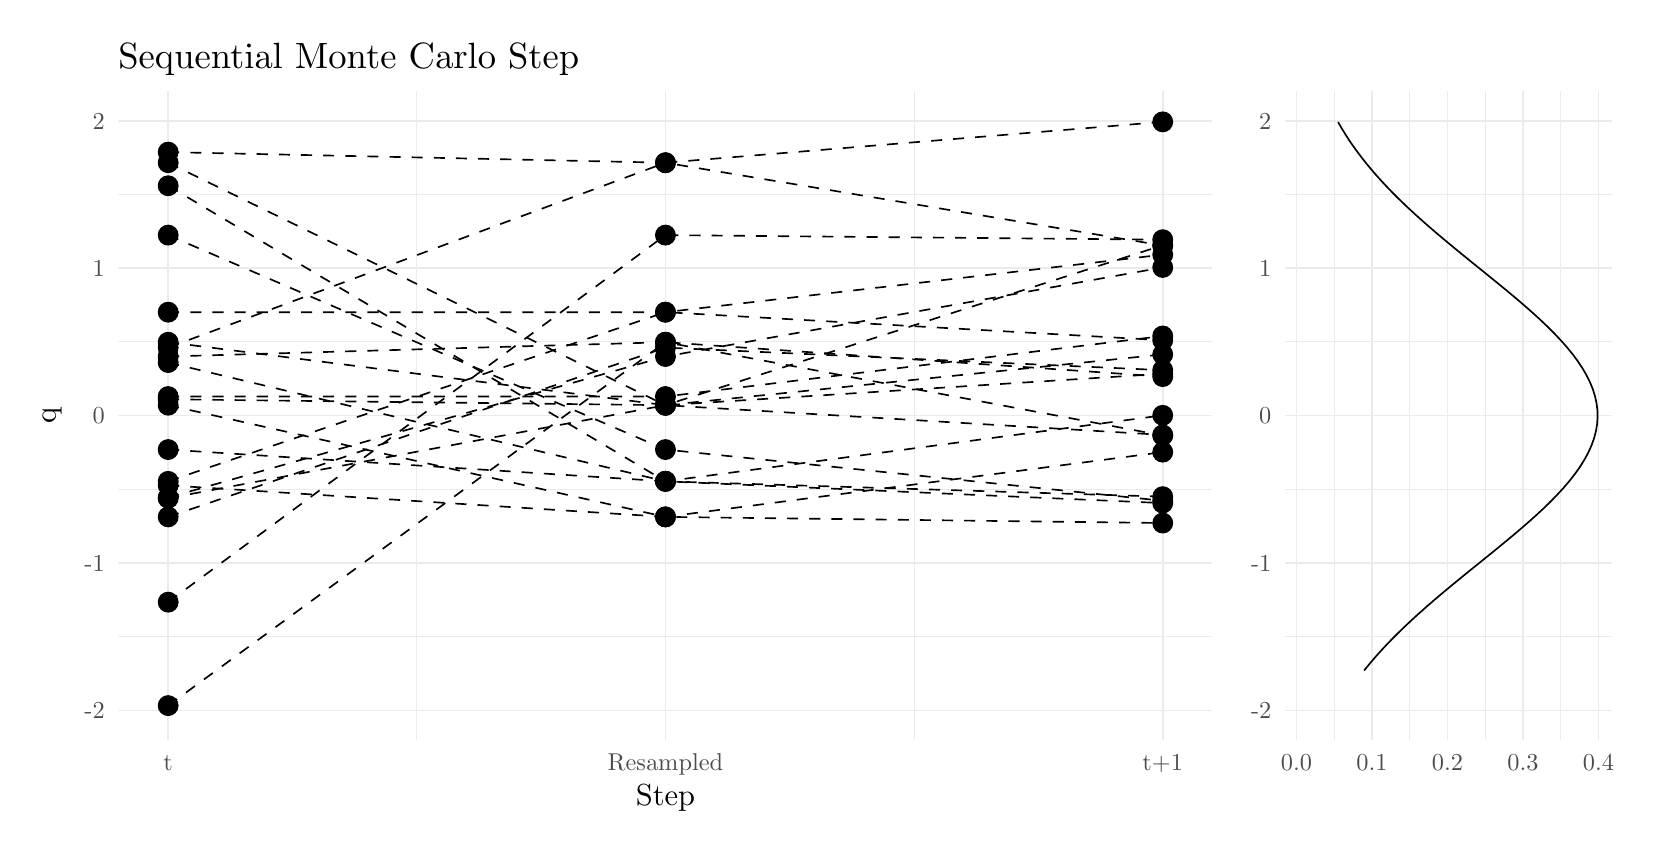
\begin{tikzpicture}[x=1pt,y=1pt]
\definecolor{fillColor}{RGB}{255,255,255}
\path[use as bounding box,fill=fillColor,fill opacity=0.00] (0,0) rectangle (578.16,289.08);
\begin{scope}
\path[clip] ( 32.80, 31.68) rectangle (428.12,266.12);
\definecolor{drawColor}{gray}{0.92}

\path[draw=drawColor,line width= 0.3pt,line join=round] ( 32.80, 68.98) --
	(428.12, 68.98);

\path[draw=drawColor,line width= 0.3pt,line join=round] ( 32.80,122.26) --
	(428.12,122.26);

\path[draw=drawColor,line width= 0.3pt,line join=round] ( 32.80,175.54) --
	(428.12,175.54);

\path[draw=drawColor,line width= 0.3pt,line join=round] ( 32.80,228.82) --
	(428.12,228.82);

\path[draw=drawColor,line width= 0.3pt,line join=round] (140.62, 31.68) --
	(140.62,266.12);

\path[draw=drawColor,line width= 0.3pt,line join=round] (320.31, 31.68) --
	(320.31,266.12);

\path[draw=drawColor,line width= 0.6pt,line join=round] ( 32.80, 42.34) --
	(428.12, 42.34);

\path[draw=drawColor,line width= 0.6pt,line join=round] ( 32.80, 95.62) --
	(428.12, 95.62);

\path[draw=drawColor,line width= 0.6pt,line join=round] ( 32.80,148.90) --
	(428.12,148.90);

\path[draw=drawColor,line width= 0.6pt,line join=round] ( 32.80,202.18) --
	(428.12,202.18);

\path[draw=drawColor,line width= 0.6pt,line join=round] ( 32.80,255.46) --
	(428.12,255.46);

\path[draw=drawColor,line width= 0.6pt,line join=round] ( 50.77, 31.68) --
	( 50.77,266.12);

\path[draw=drawColor,line width= 0.6pt,line join=round] (230.46, 31.68) --
	(230.46,266.12);

\path[draw=drawColor,line width= 0.6pt,line join=round] (410.15, 31.68) --
	(410.15,266.12);
\definecolor{drawColor}{RGB}{0,0,0}
\definecolor{fillColor}{RGB}{0,0,0}

\path[draw=drawColor,line width= 0.4pt,line join=round,line cap=round,fill=fillColor] ( 50.77,119.04) circle (  3.57);

\path[draw=drawColor,line width= 0.4pt,line join=round,line cap=round,fill=fillColor] ( 50.77,136.63) circle (  3.57);

\path[draw=drawColor,line width= 0.4pt,line join=round,line cap=round,fill=fillColor] ( 50.77,231.95) circle (  3.57);

\path[draw=drawColor,line width= 0.4pt,line join=round,line cap=round,fill=fillColor] ( 50.77,152.66) circle (  3.57);

\path[draw=drawColor,line width= 0.4pt,line join=round,line cap=round,fill=fillColor] ( 50.77,155.79) circle (  3.57);

\path[draw=drawColor,line width= 0.4pt,line join=round,line cap=round,fill=fillColor] ( 50.77,240.28) circle (  3.57);

\path[draw=drawColor,line width= 0.4pt,line join=round,line cap=round,fill=fillColor] ( 50.77,173.46) circle (  3.57);

\path[draw=drawColor,line width= 0.4pt,line join=round,line cap=round,fill=fillColor] ( 50.77, 81.49) circle (  3.57);

\path[draw=drawColor,line width= 0.4pt,line join=round,line cap=round,fill=fillColor] ( 50.77,112.30) circle (  3.57);

\path[draw=drawColor,line width= 0.4pt,line join=round,line cap=round,fill=fillColor] ( 50.77,125.15) circle (  3.57);

\path[draw=drawColor,line width= 0.4pt,line join=round,line cap=round,fill=fillColor] ( 50.77,214.12) circle (  3.57);

\path[draw=drawColor,line width= 0.4pt,line join=round,line cap=round,fill=fillColor] ( 50.77,168.07) circle (  3.57);

\path[draw=drawColor,line width= 0.4pt,line join=round,line cap=round,fill=fillColor] ( 50.77,170.25) circle (  3.57);

\path[draw=drawColor,line width= 0.4pt,line join=round,line cap=round,fill=fillColor] ( 50.77,154.80) circle (  3.57);

\path[draw=drawColor,line width= 0.4pt,line join=round,line cap=round,fill=fillColor] ( 50.77,119.28) circle (  3.57);

\path[draw=drawColor,line width= 0.4pt,line join=round,line cap=round,fill=fillColor] ( 50.77,244.11) circle (  3.57);

\path[draw=drawColor,line width= 0.4pt,line join=round,line cap=round,fill=fillColor] ( 50.77,175.42) circle (  3.57);

\path[draw=drawColor,line width= 0.4pt,line join=round,line cap=round,fill=fillColor] ( 50.77, 44.11) circle (  3.57);

\path[draw=drawColor,line width= 0.4pt,line join=round,line cap=round,fill=fillColor] ( 50.77,186.27) circle (  3.57);

\path[draw=drawColor,line width= 0.4pt,line join=round,line cap=round,fill=fillColor] ( 50.77,123.71) circle (  3.57);

\path[draw=drawColor,line width= 0.4pt,line join=round,line cap=round,fill=fillColor] (230.46,152.66) circle (  3.57);

\path[draw=drawColor,line width= 0.4pt,line join=round,line cap=round,fill=fillColor] (230.46,125.15) circle (  3.57);

\path[draw=drawColor,line width= 0.4pt,line join=round,line cap=round,fill=fillColor] (230.46,125.15) circle (  3.57);

\path[draw=drawColor,line width= 0.4pt,line join=round,line cap=round,fill=fillColor] (230.46,112.30) circle (  3.57);

\path[draw=drawColor,line width= 0.4pt,line join=round,line cap=round,fill=fillColor] (230.46,155.79) circle (  3.57);

\path[draw=drawColor,line width= 0.4pt,line join=round,line cap=round,fill=fillColor] (230.46,152.66) circle (  3.57);

\path[draw=drawColor,line width= 0.4pt,line join=round,line cap=round,fill=fillColor] (230.46,240.28) circle (  3.57);

\path[draw=drawColor,line width= 0.4pt,line join=round,line cap=round,fill=fillColor] (230.46,214.12) circle (  3.57);

\path[draw=drawColor,line width= 0.4pt,line join=round,line cap=round,fill=fillColor] (230.46,173.46) circle (  3.57);

\path[draw=drawColor,line width= 0.4pt,line join=round,line cap=round,fill=fillColor] (230.46,186.27) circle (  3.57);

\path[draw=drawColor,line width= 0.4pt,line join=round,line cap=round,fill=fillColor] (230.46,136.63) circle (  3.57);

\path[draw=drawColor,line width= 0.4pt,line join=round,line cap=round,fill=fillColor] (230.46,125.15) circle (  3.57);

\path[draw=drawColor,line width= 0.4pt,line join=round,line cap=round,fill=fillColor] (230.46,175.42) circle (  3.57);

\path[draw=drawColor,line width= 0.4pt,line join=round,line cap=round,fill=fillColor] (230.46,152.66) circle (  3.57);

\path[draw=drawColor,line width= 0.4pt,line join=round,line cap=round,fill=fillColor] (230.46,170.25) circle (  3.57);

\path[draw=drawColor,line width= 0.4pt,line join=round,line cap=round,fill=fillColor] (230.46,240.28) circle (  3.57);

\path[draw=drawColor,line width= 0.4pt,line join=round,line cap=round,fill=fillColor] (230.46,152.66) circle (  3.57);

\path[draw=drawColor,line width= 0.4pt,line join=round,line cap=round,fill=fillColor] (230.46,175.42) circle (  3.57);

\path[draw=drawColor,line width= 0.4pt,line join=round,line cap=round,fill=fillColor] (230.46,186.27) circle (  3.57);

\path[draw=drawColor,line width= 0.4pt,line join=round,line cap=round,fill=fillColor] (230.46,112.30) circle (  3.57);

\path[draw=drawColor,line width= 0.4pt,line join=round,line cap=round,fill=fillColor] (410.15,164.02) circle (  3.57);

\path[draw=drawColor,line width= 0.4pt,line join=round,line cap=round,fill=fillColor] (410.15,117.29) circle (  3.57);

\path[draw=drawColor,line width= 0.4pt,line join=round,line cap=round,fill=fillColor] (410.15,149.00) circle (  3.57);

\path[draw=drawColor,line width= 0.4pt,line join=round,line cap=round,fill=fillColor] (410.15,135.70) circle (  3.57);

\path[draw=drawColor,line width= 0.4pt,line join=round,line cap=round,fill=fillColor] (410.15,177.67) circle (  3.57);

\path[draw=drawColor,line width= 0.4pt,line join=round,line cap=round,fill=fillColor] (410.15,171.00) circle (  3.57);

\path[draw=drawColor,line width= 0.4pt,line join=round,line cap=round,fill=fillColor] (410.15,255.04) circle (  3.57);

\path[draw=drawColor,line width= 0.4pt,line join=round,line cap=round,fill=fillColor] (410.15,212.47) circle (  3.57);

\path[draw=drawColor,line width= 0.4pt,line join=round,line cap=round,fill=fillColor] (410.15,165.31) circle (  3.57);

\path[draw=drawColor,line width= 0.4pt,line join=round,line cap=round,fill=fillColor] (410.15,176.13) circle (  3.57);

\path[draw=drawColor,line width= 0.4pt,line join=round,line cap=round,fill=fillColor] (410.15,118.13) circle (  3.57);

\path[draw=drawColor,line width= 0.4pt,line join=round,line cap=round,fill=fillColor] (410.15,119.61) circle (  3.57);

\path[draw=drawColor,line width= 0.4pt,line join=round,line cap=round,fill=fillColor] (410.15,141.71) circle (  3.57);

\path[draw=drawColor,line width= 0.4pt,line join=round,line cap=round,fill=fillColor] (410.15,210.44) circle (  3.57);

\path[draw=drawColor,line width= 0.4pt,line join=round,line cap=round,fill=fillColor] (410.15,202.43) circle (  3.57);

\path[draw=drawColor,line width= 0.4pt,line join=round,line cap=round,fill=fillColor] (410.15,210.36) circle (  3.57);

\path[draw=drawColor,line width= 0.4pt,line join=round,line cap=round,fill=fillColor] (410.15,141.92) circle (  3.57);

\path[draw=drawColor,line width= 0.4pt,line join=round,line cap=round,fill=fillColor] (410.15,162.99) circle (  3.57);

\path[draw=drawColor,line width= 0.4pt,line join=round,line cap=round,fill=fillColor] (410.15,207.05) circle (  3.57);

\path[draw=drawColor,line width= 0.4pt,line join=round,line cap=round,fill=fillColor] (410.15,110.08) circle (  3.57);

\path[draw=drawColor,line width= 0.6pt,dash pattern=on 4pt off 4pt ,line join=round] ( 50.77,119.04) --
	(230.46,152.66) --
	(410.15,164.02);

\path[draw=drawColor,line width= 0.6pt,dash pattern=on 4pt off 4pt ,line join=round] ( 50.77,136.63) --
	(230.46,125.15) --
	(410.15,117.29);

\path[draw=drawColor,line width= 0.6pt,dash pattern=on 4pt off 4pt ,line join=round] ( 50.77,231.95) --
	(230.46,125.15) --
	(410.15,149.00);

\path[draw=drawColor,line width= 0.6pt,dash pattern=on 4pt off 4pt ,line join=round] ( 50.77,152.66) --
	(230.46,112.30) --
	(410.15,135.70);

\path[draw=drawColor,line width= 0.6pt,dash pattern=on 4pt off 4pt ,line join=round] ( 50.77,155.79) --
	(230.46,155.79) --
	(410.15,177.67);

\path[draw=drawColor,line width= 0.6pt,dash pattern=on 4pt off 4pt ,line join=round] ( 50.77,240.28) --
	(230.46,152.66) --
	(410.15,171.00);

\path[draw=drawColor,line width= 0.6pt,dash pattern=on 4pt off 4pt ,line join=round] ( 50.77,173.46) --
	(230.46,240.28) --
	(410.15,255.04);

\path[draw=drawColor,line width= 0.6pt,dash pattern=on 4pt off 4pt ,line join=round] ( 50.77, 81.49) --
	(230.46,214.12) --
	(410.15,212.47);

\path[draw=drawColor,line width= 0.6pt,dash pattern=on 4pt off 4pt ,line join=round] ( 50.77,112.30) --
	(230.46,173.46) --
	(410.15,165.31);

\path[draw=drawColor,line width= 0.6pt,dash pattern=on 4pt off 4pt ,line join=round] ( 50.77,125.15) --
	(230.46,186.27) --
	(410.15,176.13);

\path[draw=drawColor,line width= 0.6pt,dash pattern=on 4pt off 4pt ,line join=round] ( 50.77,214.12) --
	(230.46,136.63) --
	(410.15,118.13);

\path[draw=drawColor,line width= 0.6pt,dash pattern=on 4pt off 4pt ,line join=round] ( 50.77,168.07) --
	(230.46,125.15) --
	(410.15,119.61);

\path[draw=drawColor,line width= 0.6pt,dash pattern=on 4pt off 4pt ,line join=round] ( 50.77,170.25) --
	(230.46,175.42) --
	(410.15,141.71);

\path[draw=drawColor,line width= 0.6pt,dash pattern=on 4pt off 4pt ,line join=round] ( 50.77,154.80) --
	(230.46,152.66) --
	(410.15,210.44);

\path[draw=drawColor,line width= 0.6pt,dash pattern=on 4pt off 4pt ,line join=round] ( 50.77,119.28) --
	(230.46,170.25) --
	(410.15,202.43);

\path[draw=drawColor,line width= 0.6pt,dash pattern=on 4pt off 4pt ,line join=round] ( 50.77,244.11) --
	(230.46,240.28) --
	(410.15,210.36);

\path[draw=drawColor,line width= 0.6pt,dash pattern=on 4pt off 4pt ,line join=round] ( 50.77,175.42) --
	(230.46,152.66) --
	(410.15,141.92);

\path[draw=drawColor,line width= 0.6pt,dash pattern=on 4pt off 4pt ,line join=round] ( 50.77, 44.11) --
	(230.46,175.42) --
	(410.15,162.99);

\path[draw=drawColor,line width= 0.6pt,dash pattern=on 4pt off 4pt ,line join=round] ( 50.77,186.27) --
	(230.46,186.27) --
	(410.15,207.05);

\path[draw=drawColor,line width= 0.6pt,dash pattern=on 4pt off 4pt ,line join=round] ( 50.77,123.71) --
	(230.46,112.30) --
	(410.15,110.08);
\end{scope}
\begin{scope}
\path[clip] (  0.00,  0.00) rectangle (578.16,289.08);
\definecolor{drawColor}{gray}{0.30}

\node[text=drawColor,anchor=base east,inner sep=0pt, outer sep=0pt, scale=  0.88] at ( 27.85, 39.30) {-2};

\node[text=drawColor,anchor=base east,inner sep=0pt, outer sep=0pt, scale=  0.88] at ( 27.85, 92.59) {-1};

\node[text=drawColor,anchor=base east,inner sep=0pt, outer sep=0pt, scale=  0.88] at ( 27.85,145.87) {0};

\node[text=drawColor,anchor=base east,inner sep=0pt, outer sep=0pt, scale=  0.88] at ( 27.85,199.15) {1};

\node[text=drawColor,anchor=base east,inner sep=0pt, outer sep=0pt, scale=  0.88] at ( 27.85,252.43) {2};
\end{scope}
\begin{scope}
\path[clip] (  0.00,  0.00) rectangle (578.16,289.08);
\definecolor{drawColor}{gray}{0.30}

\node[text=drawColor,anchor=base,inner sep=0pt, outer sep=0pt, scale=  0.88] at ( 50.77, 20.67) {t};

\node[text=drawColor,anchor=base,inner sep=0pt, outer sep=0pt, scale=  0.88] at (230.46, 20.67) {Resampled};

\node[text=drawColor,anchor=base,inner sep=0pt, outer sep=0pt, scale=  0.88] at (410.15, 20.67) {t+1};
\end{scope}
\begin{scope}
\path[clip] (  0.00,  0.00) rectangle (578.16,289.08);
\definecolor{drawColor}{RGB}{0,0,0}

\node[text=drawColor,anchor=base,inner sep=0pt, outer sep=0pt, scale=  1.10] at (230.46,  7.93) {Step};
\end{scope}
\begin{scope}
\path[clip] (  0.00,  0.00) rectangle (578.16,289.08);
\definecolor{drawColor}{RGB}{0,0,0}

\node[text=drawColor,rotate= 90.00,anchor=base west,inner sep=0pt, outer sep=0pt, scale=  1.10] at ( 10.23,146.00) {q};
\end{scope}
\begin{scope}
\path[clip] (  0.00,  0.00) rectangle (578.16,289.08);
\definecolor{drawColor}{RGB}{0,0,0}

\node[text=drawColor,anchor=base west,inner sep=0pt, outer sep=0pt, scale=  1.32] at ( 32.80,274.49) {Sequential Monte Carlo Step};
\end{scope}
\begin{scope}
\path[clip] (454.37, 31.68) rectangle (572.66,266.12);
\definecolor{drawColor}{gray}{0.92}

\path[draw=drawColor,line width= 0.3pt,line join=round] (454.37, 68.98) --
	(572.66, 68.98);

\path[draw=drawColor,line width= 0.3pt,line join=round] (454.37,122.26) --
	(572.66,122.26);

\path[draw=drawColor,line width= 0.3pt,line join=round] (454.37,175.54) --
	(572.66,175.54);

\path[draw=drawColor,line width= 0.3pt,line join=round] (454.37,228.82) --
	(572.66,228.82);

\path[draw=drawColor,line width= 0.3pt,line join=round] (472.14, 31.68) --
	(472.14,266.12);

\path[draw=drawColor,line width= 0.3pt,line join=round] (499.41, 31.68) --
	(499.41,266.12);

\path[draw=drawColor,line width= 0.3pt,line join=round] (526.68, 31.68) --
	(526.68,266.12);

\path[draw=drawColor,line width= 0.3pt,line join=round] (553.95, 31.68) --
	(553.95,266.12);

\path[draw=drawColor,line width= 0.6pt,line join=round] (454.37, 42.34) --
	(572.66, 42.34);

\path[draw=drawColor,line width= 0.6pt,line join=round] (454.37, 95.62) --
	(572.66, 95.62);

\path[draw=drawColor,line width= 0.6pt,line join=round] (454.37,148.90) --
	(572.66,148.90);

\path[draw=drawColor,line width= 0.6pt,line join=round] (454.37,202.18) --
	(572.66,202.18);

\path[draw=drawColor,line width= 0.6pt,line join=round] (454.37,255.46) --
	(572.66,255.46);

\path[draw=drawColor,line width= 0.6pt,line join=round] (458.51, 31.68) --
	(458.51,266.12);

\path[draw=drawColor,line width= 0.6pt,line join=round] (485.78, 31.68) --
	(485.78,266.12);

\path[draw=drawColor,line width= 0.6pt,line join=round] (513.04, 31.68) --
	(513.04,266.12);

\path[draw=drawColor,line width= 0.6pt,line join=round] (540.31, 31.68) --
	(540.31,266.12);

\path[draw=drawColor,line width= 0.6pt,line join=round] (567.58, 31.68) --
	(567.58,266.12);
\definecolor{drawColor}{RGB}{0,0,0}

\path[draw=drawColor,line width= 0.6pt,line join=round] (482.93, 56.80) --
	(485.00, 59.34) --
	(487.17, 61.88) --
	(489.46, 64.42) --
	(491.85, 66.96) --
	(494.35, 69.50) --
	(496.95, 72.04) --
	(499.64, 74.58) --
	(502.41, 77.12) --
	(505.27, 79.66) --
	(508.21, 82.21) --
	(511.20, 84.75) --
	(514.25, 87.29) --
	(517.35, 89.83) --
	(520.47, 92.37) --
	(523.61, 94.91) --
	(526.76, 97.45) --
	(529.89, 99.99) --
	(533.00,102.53) --
	(536.07,105.07) --
	(539.08,107.61) --
	(542.02,110.15) --
	(544.86,112.69) --
	(547.61,115.23) --
	(550.23,117.77) --
	(552.71,120.31) --
	(555.04,122.85) --
	(557.21,125.40) --
	(559.19,127.94) --
	(560.98,130.48) --
	(562.56,133.02) --
	(563.93,135.56) --
	(565.08,138.10) --
	(565.99,140.64) --
	(566.67,143.18) --
	(567.10,145.72) --
	(567.28,148.26) --
	(567.22,150.80) --
	(566.91,153.34) --
	(566.36,155.88) --
	(565.57,158.42) --
	(564.54,160.96) --
	(563.28,163.50) --
	(561.80,166.04) --
	(560.11,168.59) --
	(558.23,171.13) --
	(556.15,173.67) --
	(553.90,176.21) --
	(551.49,178.75) --
	(548.94,181.29) --
	(546.26,183.83) --
	(543.46,186.37) --
	(540.56,188.91) --
	(537.59,191.45) --
	(534.55,193.99) --
	(531.46,196.53) --
	(528.33,199.07) --
	(525.19,201.61) --
	(522.04,204.15) --
	(518.91,206.69) --
	(515.80,209.24) --
	(512.73,211.78) --
	(509.70,214.32) --
	(506.74,216.86) --
	(503.84,219.40) --
	(501.02,221.94) --
	(498.28,224.48) --
	(495.64,227.02) --
	(493.09,229.56) --
	(490.65,232.10) --
	(488.31,234.64) --
	(486.08,237.18) --
	(483.95,239.72) --
	(481.94,242.26) --
	(480.04,244.80) --
	(478.24,247.34) --
	(476.56,249.88) --
	(474.98,252.43) --
	(473.51,254.97);
\end{scope}
\begin{scope}
\path[clip] (  0.00,  0.00) rectangle (578.16,289.08);
\definecolor{drawColor}{gray}{0.30}

\node[text=drawColor,anchor=base east,inner sep=0pt, outer sep=0pt, scale=  0.88] at (449.42, 39.30) {-2};

\node[text=drawColor,anchor=base east,inner sep=0pt, outer sep=0pt, scale=  0.88] at (449.42, 92.59) {-1};

\node[text=drawColor,anchor=base east,inner sep=0pt, outer sep=0pt, scale=  0.88] at (449.42,145.87) {0};

\node[text=drawColor,anchor=base east,inner sep=0pt, outer sep=0pt, scale=  0.88] at (449.42,199.15) {1};

\node[text=drawColor,anchor=base east,inner sep=0pt, outer sep=0pt, scale=  0.88] at (449.42,252.43) {2};
\end{scope}
\begin{scope}
\path[clip] (  0.00,  0.00) rectangle (578.16,289.08);
\definecolor{drawColor}{gray}{0.30}

\node[text=drawColor,anchor=base,inner sep=0pt, outer sep=0pt, scale=  0.88] at (458.51, 20.67) {0.0};

\node[text=drawColor,anchor=base,inner sep=0pt, outer sep=0pt, scale=  0.88] at (485.78, 20.67) {0.1};

\node[text=drawColor,anchor=base,inner sep=0pt, outer sep=0pt, scale=  0.88] at (513.04, 20.67) {0.2};

\node[text=drawColor,anchor=base,inner sep=0pt, outer sep=0pt, scale=  0.88] at (540.31, 20.67) {0.3};

\node[text=drawColor,anchor=base,inner sep=0pt, outer sep=0pt, scale=  0.88] at (567.58, 20.67) {0.4};
\end{scope}
\end{tikzpicture}

